% !TeX option = --shell-escape
\documentclass[11pt]{article}

%page borders and line spacing
\linespread{1.4}
\usepackage[a4paper, total={6in, 10in}]{geometry}

%custom commands and packages
\usepackage{tex/preamble/packages}
\usepackage{tex/preamble/commands}

\pagestyle{fancy}
\fancyhf{}
\lfoot{Computational High Energy Physics}
\rfoot{2025 University of Bern}
\cfoot{\thepage}

\begin{document}

\begin{titlepage}
   \begin{center}
       \vspace*{3cm}
        \Huge
       \textbf{Computational High Energy Physics}
       
       \vspace{0.5cm}
         \LARGE
       \vspace{1cm}
%      \textbf{Jesse Woods}
       \vfill
    \vspace{2cm}
       \vfill
             \Large
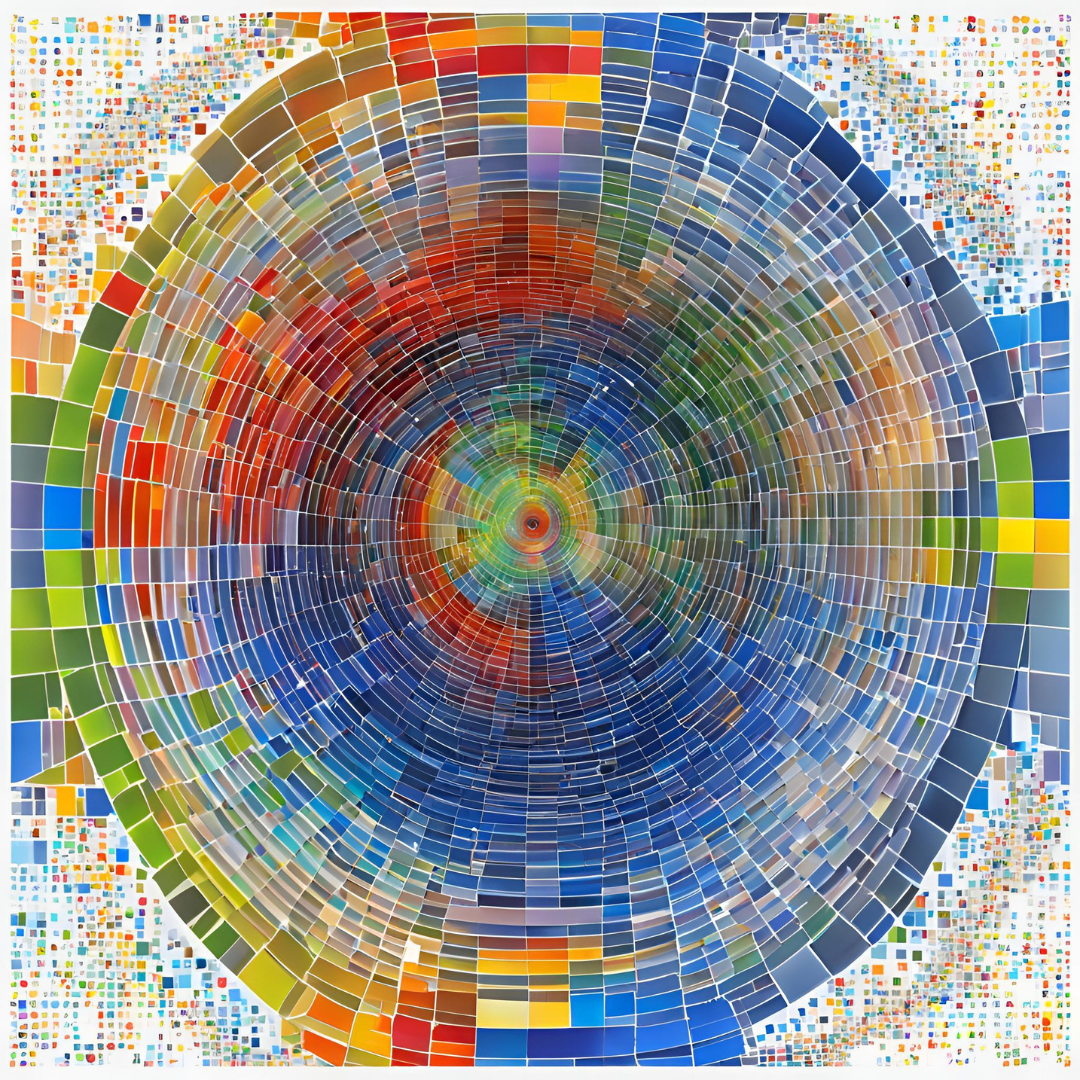
\includegraphics[width=0.8\textwidth]{tex/ims/numcol.png}
       \vspace{0.8cm}
       % Department of Applied Mathematics and Theoretical Physics\\
       % University of Cambridge\\
       % United Kingdom \\
       % April 2024       
   \end{center}
\end{titlepage}


\tableofcontents
\newpage


\section{Introduction}

These notes follow the course `Computational High Energy Physics' offered by Prof. Dr. Valentin Hirschi in 2025 at the University of Bern. It covers theoretical aspects of implementing a numerical collider in an efficient way, as well as a practical component implementing the various pieces required in order to simulate high energy collisions of the likes at CERN.



\newpage

\section*{Lecture 1: Differential Cross-Sections at Fixed Order
}

\newpage


\section*{Practical 1: Installing Ubuntu, MadGraph5, and Testing with Python}
\addcontentsline{toc}{section}{Practical 1: Installing Ubuntu, MadGraph5, and Testing with Python}


\subsection*{Setup}
To begin with, we will need a working Linux operating system installed on our computer. If you're a Windows user, the easiest way to do this is by using the official Windows  Subsystem for Linux (WSL), where the instructions to install can be found \href{https://learn.microsoft.com/en-us/windows/wsl/install}{here}. Once installed, you should be able to run the program Ubuntu, which will open a command prompt Window which allows you to interact with the copy of Ubuntu now running on your computer.

To test to see if your installation is working, you can run the command \codeinline{ls} to list the contents of the current directory. This will be empty, but should run without errors. You can then make a new folder (directory) named `chep' by running
\begin{codeenv}
    mkdir chep
\end{codeenv}
If you run \codeinline{ls} again, you should now see this folder in the output. To move into this folder, we can change directory
\begin{codeenv}
    cd chep
\end{codeenv}
Next, check to make sure Git is installed, by running
\begin{codeenv}
    which git
\end{codeenv}
This should tell you where your git installation is. If this doesn't work, make sure git is installed.
If this runs without problem we should be able download the latest version of the course repository by running
\begin{codeenv}
    git clone https://github.com/ValentinHirschi/ComputationalHEP.git 
\end{codeenv}
and navigate into its directory
\begin{codeenv}
    cd ComputationalHEP/  
\end{codeenv}
We can run \codeinline{ls} to see the newly downloaded contents. We can also update this repository week by week by using
\begin{codeenv}
    git pull
\end{codeenv}

To edit the code for the course, the simplest way is to use VS Code. To open the repository in VS Code, we can run from the current directory
\begin{codeenv}
    code .
\end{codeenv}
This should install and open a VS Code window.

Along with our course code, we will also be running MadGraph5. We install this using
\begin{codeenv}
     wget https://launchpad.net/mg5amcnlo/3.0/3.6.x/+download/MG5_aMC_v3.5.7.tar.gz
\end{codeenv}
We can unpack this tarball using
\begin{codeenv}
     tar -xzf MG5_aMC_v3.5.7.tar.gz
\end{codeenv}
We should now see the decompressed contents when we run \codeinline{ls}. We can then remove the zipped file, as we no longer need it
\begin{codeenv}
     rm -rf MG5_aMC_v3.5.7.tar.gz
\end{codeenv}
We will now have a new directory that we can navigate into
\begin{codeenv}
     cd MG5_aMC_v3_5_7/
\end{codeenv}

We will also need few other things installed to get everything to run properly. To ensure this works, first run
\begin{codeenv}
   sudo apt-get update
\end{codeenv}
and enter your password when prompted. Then, we need to install Fortran
\begin{codeenv}
     sudo apt update && sudo apt-get install gfortran
\end{codeenv}
and type \codeinline{Y} to proceed. We also need C++ installed, which can be done with
\begin{codeenv}
     sudo apt install build-essential
\end{codeenv}

For our python code that we will run later, we will also need a few packages. Firstly, check \codeinline{python3 --version}, and make sure it is $\geq 3.12$. If not, run
\begin{codeenv}
   sudo add-apt-repository ppa:deadsnakes/ppa -y 
   sudo apt update 
   sudo apt install -y python3.12 python3.12-venv python3.12-dev 
   sudo update-alternatives --install /usr/bin/python3 python3 /usr/bin/python3.12 1 
   sudo update-alternatives --config python3
\end{codeenv}
To install packages, we need to use \codeinline{pip}. To install this, run % sudo apt install python3.12-venv
\begin{codeenv}
    sudo apt install python3-pip
    python3 -m ensurepip --upgrade 
    python3 -m pip install --upgrade pip setuptools
\end{codeenv}
Then, we install \codeinline{symbolica}
\begin{codeenv}
    pip install symbolica
\end{codeenv}
and \codeinline{numpy}
\begin{codeenv}
    pip install numpy
\end{codeenv}

\subsection*{Our First Process in Madgraph}
Lets try and use Madgraph, and see how it works. To run it, use the command
\begin{codeenv}
    ./bin/mg5_aMC
\end{codeenv}
You should now see the introduction text for MadGraph5. To see the commands that are part of the package, we can type
\begin{codeenv}
    help
\end{codeenv}
If you ever get stuck, you can use the \codeinline{help} command to view documentation and instructions.
Lets try and generate the cross section for a simple process, $e^+e^-\to \mu^+\mu^-$. To do this, we will generate the process:
\begin{codeenv}
    generate e+ e- > mu+ mu-
\end{codeenv}
The output should say that we have generated one process with two diagrams. These will correspond to scattering via an intermediate photon, and intermediate $Z$ boson. To see these, we can run
\begin{codeenv}
    display diagrams ./
\end{codeenv}
This  will generate a file with a drawing of the diagrams (you may not be able to open it though on the default Windows installation).

Obviously, if we want to study Quantum Electrodynamics, we don't want to consider the process mediated by the $Z$ boson. We can ignore this process by using instead

\begin{codeenv}
    generate e+ e- > mu+ mu- / z
\end{codeenv}

To compute the result, we can firstly output the process
\begin{codeenv}
    output
\end{codeenv}
and then begin by typing
\begin{codeenv}
    launch
\end{codeenv}
This will begin running the code. We can choose now to adjust some parameters (we have 60 seconds to decide if we want to do this). We won't adjust any of the first options for now, so enter \codeinline{0}. On the next screen, we would like to edit some run paramters, so enter \codeinline{2}. This will enter an editor window. You can navigate the text using the arrow keys. To edit the text, we enter `insert' mode by pressing \codeinline{i}. To stop editing, press \codeinline{Esc}. To save and exit this screen, type \codeinline{:w} to write your edits, then \codeinline{:q} to exit to the previous screen. 

We would like to make a few edits. 

Firstly, in the Standard Cuts section, we would like to remove the cutoffs. We should set also \codeinline{ptl}, the minimum, to \codeinline{0.0}.

We would also like to set the remove the upper bound on rapidity by setting \codeinline{etal} to \codeinline{-1}.

We will also remove the minimum distance between leptons by setting \codeinline{drll} to \codeinline{0.0}.

You can then exit to the previous screen, and run the process by entering \codeinline{0}. This will run and produce a numerical calculation of the cross-section! It should be something like
\begin{codeenv}
     Cross-section :   0.09286 +- 2.585e-05 pb
\end{codeenv}

We can now exit Madgraph by typing
\begin{codeenv}
    exit
\end{codeenv}

\subsection*{Our First Process in Python}

The course code we downloaded contains a Python script that we can use to compute the same process. Lets navigate back up to the project directory with \codeinline{cd ..} to where our python code will be. Lets open again VS Code by typing \codeinline{code .}. Inside the \codeinline{experiments} folder, there is a file called \codeinline{epem_lplm_fixed_order_LO.py}. This is a Python script that implements the same scattering process that we just computed in MadGraph. We will be trying to understand exactly what this code does, and how to modify it to model processes other than leptonic processes $e^+ e^- \to l^+l^-$.

Let's first trying running the code as it is. To see how to do this, we can firstly go back to the terminal, and run
\begin{codeenv}
    ./run.py --help
\end{codeenv}
This will give us some documentation. It tells us we can run the experiment \codeinline{epem_lplm_fixed_order_LO}. Let's do this
\begin{codeenv}
    ./run.py epem_lplm_fixed_order_LO --seed 3
\end{codeenv}
Here, for testing purposes, we specify the random number seed to use in order to get the same result each time. You should see the code run for a few iterations and produce a numerical result for the cross-section, for example
\begin{codeenv}
     Iteration 9: 0.0929257 +- 0.000163142, chi=1.1246
\end{codeenv}
This is quite close to the Madgraph value, indeed they lie within each others uncertainty bounds.
%Iteration 9: 0.0927061 +- 0.000160708, chi=0.630556




\section*{Lecture 2: Phase Space Sampling and Cross-Section Perturbative Expansion}

\section*{Practical 2: Implementing a Phase Space Sampler}
\addcontentsline{toc}{section}{Practical 2:  Implementing a Phase Space Sampler}


This week we will look at how phase space sampling can be implemented in python. We can begin by updating our repository with 
\begin{codeenv}
    git pull
\end{codeenv}
Make sure you're in the project directory when running this, else you'll get an error. If things aren't working (because you've done some edits), you can run
\begin{codeenv}
    git stash
\end{codeenv}
the stash away your changes. You can now \codeinline{git pull} again to get the latest version. You can then resync your changes on top of the new version using \codeinline{git stash apply}.
In the experiments folder, you should now have a new file, \codeinline{sampling_experiment.py}.
You should now also see that \codeinline{run.py} has been edited with a new case in \codeinline{__main__} for the sampling experiment. If we try and run this now, we might find that we're missing dependencies. To add the missing requirements, we can use the requirements file supplied by the repository:
\begin{codeenv}
    python3 -m pip install -r ./CHEP/requirements.txt
\end{codeenv}
Lets run the new experiment. To see how to use the new code, we can run
\begin{codeenv}
    python3 run.py sampling_experiment --help
\end{codeenv}
This tells us that we have optional run parameters which allows us to specify our random seed. Lets just run the code without a seed. If we wait a moment, we should see some lovely distributions similar to what we have seen in lectures! If the plots don't show (\codeinline{* UserWarning: FigureCanvasAgg is non-interactive}), try running 
\begin{codeenv}
    sudo apt-get install python3-tk
\end{codeenv}

\begin{figure}[H]
    \centering
    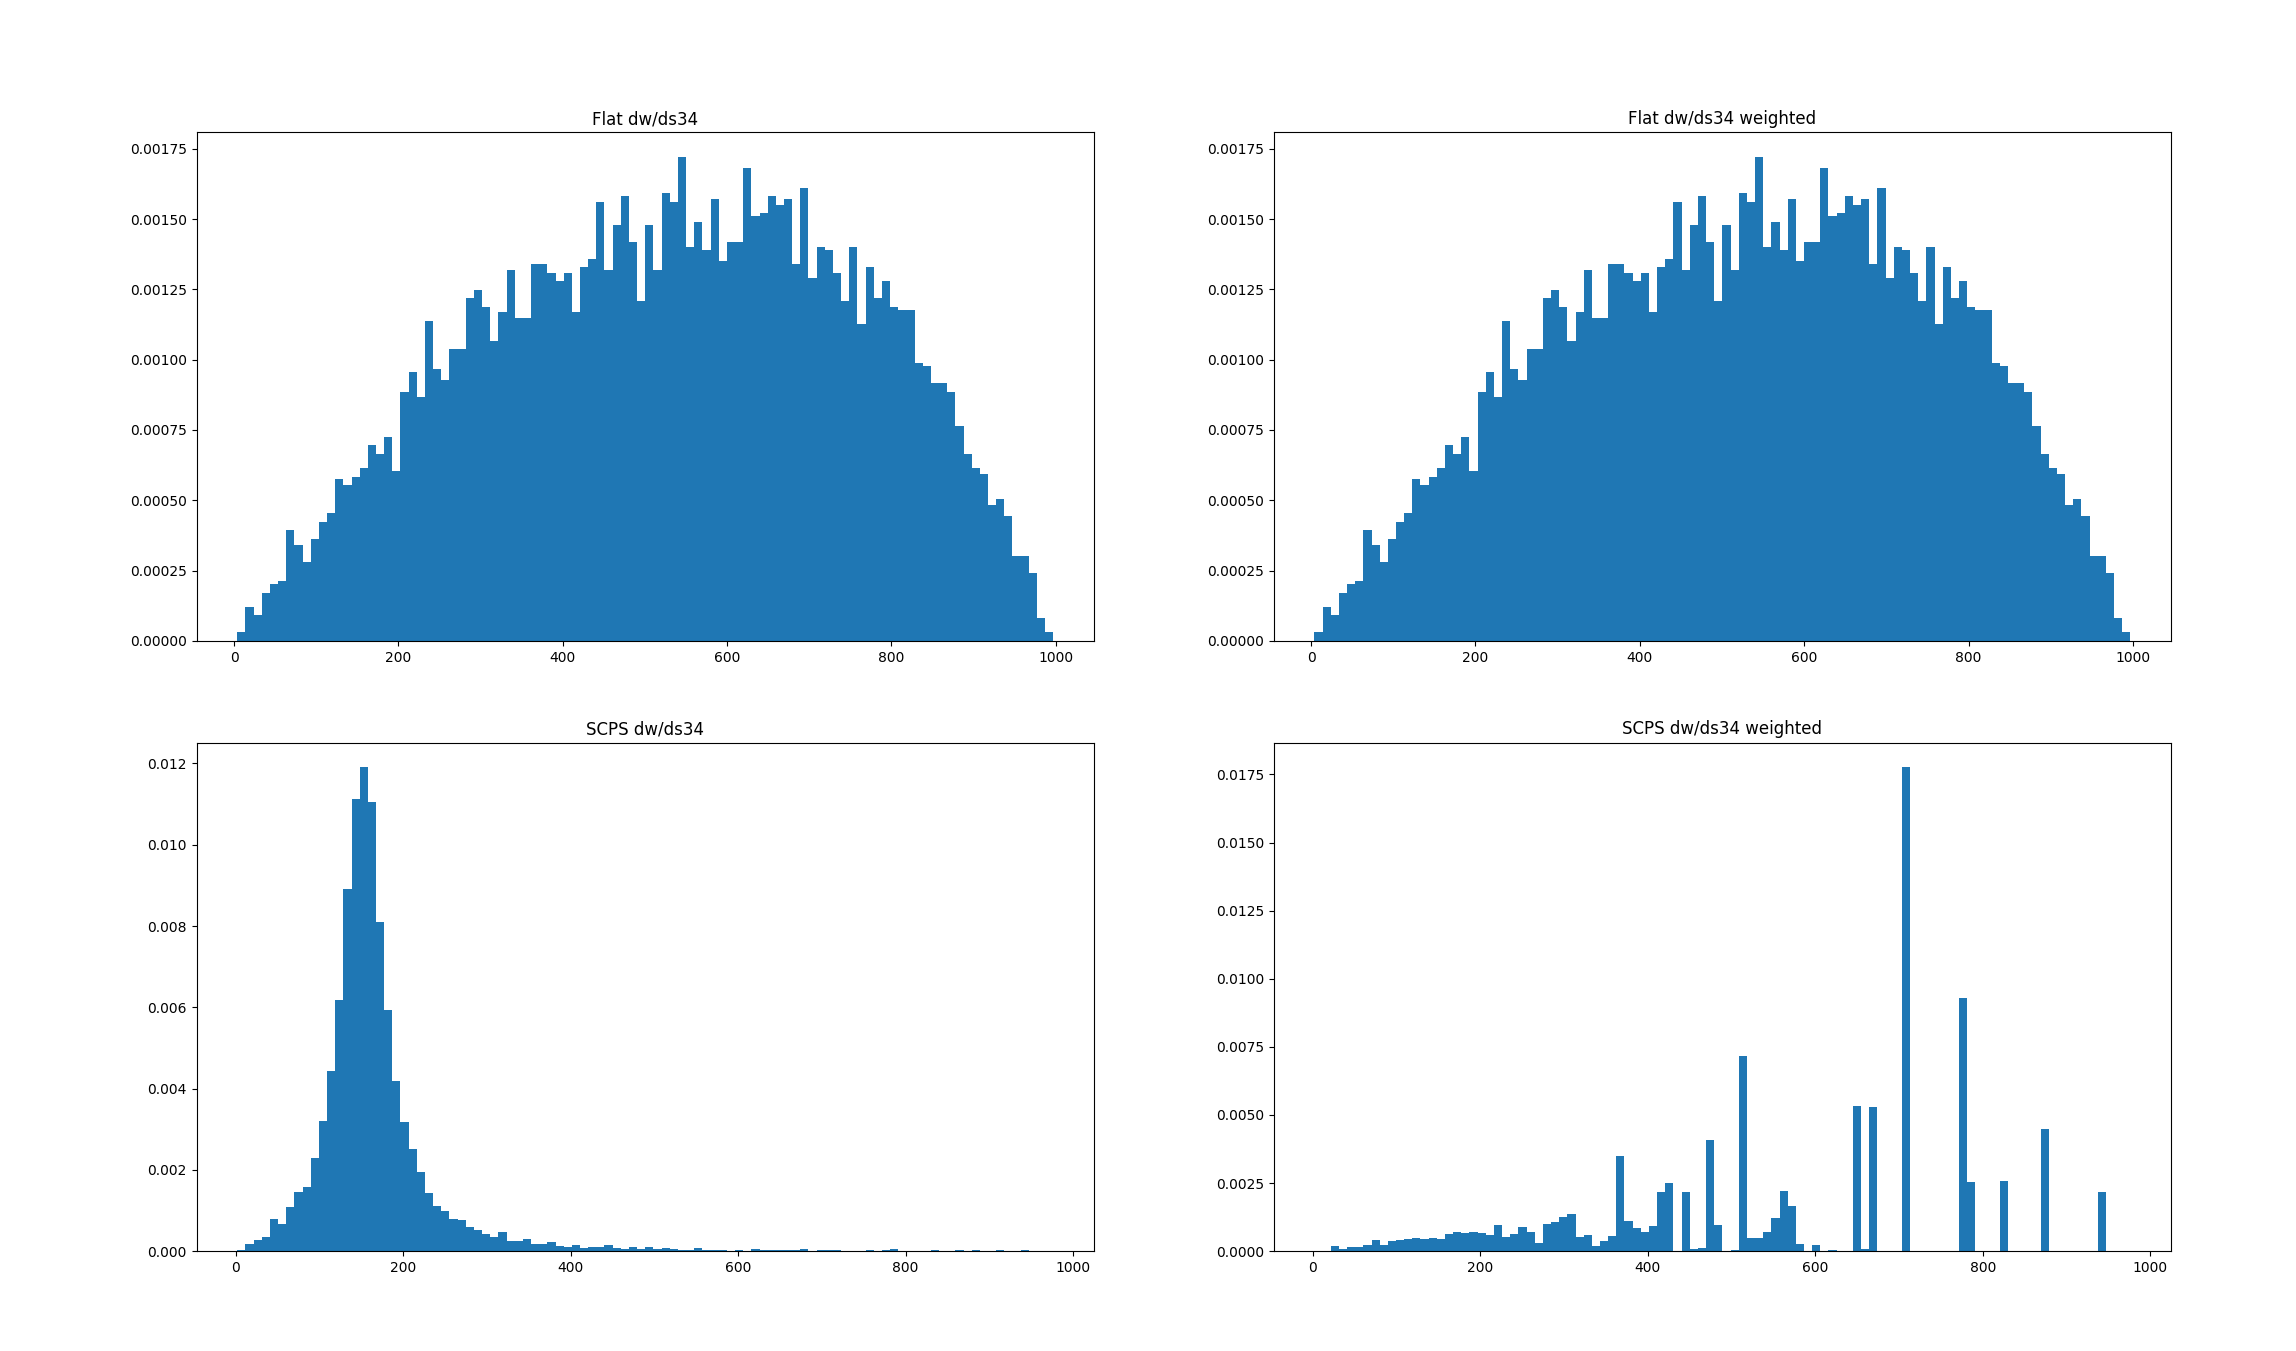
\includegraphics[width=0.75\linewidth]{tex/ims/phasespace1.png}
    \caption{Phase Space Sampling. The top row is ``flat space", so the right image is the left multiplied by the Jacobian which is just a constant (``$1$" for a normalised volume). The bottom row is biased sampling, to pick momenta distributed around the relevant pole of our process, in this case the $Z$ boson with mass 150GeV and width 60GeV.}
    \label{fig:enter-label}
\end{figure}


Lets try and understand what we're looking at, and what the code is doing. Lets open VSCode with \codeinline{code .}. Inside \codeinline{sampling_experiment}, firstly, the code picks a model. It then specifies the \codeinline{topology} - this corresponds to an assignment of momenta to our diagram.
\begin{center}
    \begin{tikzpicture}
    \begin{feynman}
        % Define vertices
        \vertex (e1) at (-3, 1) {\(e^-, p_{-3}\)};
        \vertex (e2) at (-3, -1) {\(e^+,  p_1\)};
        \vertex (v1) at (-1, 0.5) {};
        \vertex (v2) at (-1, -0.5) {};
        \vertex (v3) at (0,0.5);
        \vertex (mu1) at (2,1) {\(\mu^+,p_3\)};
        \vertex (mu2) at (2,0) {\(\mu^-,p_4\)};
        \vertex (photon) at (2, -1) {\(\gamma,p_5\)};

        % Define diagram
        \diagram* {
            (e1) -- [fermion] (v1) -- [fermion , edge label={$p_{-2}$}] (v2),
            (e2) -- [anti fermion] (v2),
            (v1) -- [boson, edge label={\(Z,\) $p_{-1}$}] (v3),
            (v3) -- [fermion] (mu2),
            (v3) -- [anti fermion] (mu1),
            (v2) -- [photon] (photon), % Initial-state radiation from the electron
        };
    \end{feynman}
\end{tikzpicture}
\end{center}

We have a propagator with momentum $p_1-p_5$ (t-channel). We also have an $s-$channel block. This is specified for our particular process in \codeinline{get_topology()}. You can \codeinline{Ctrl+Click} on  \codeinline{get_topology()} to see the assignment explicitly. Inside this function, for the outgoing $s-$channel,  we assign momentum 3 to particle ID $-12$ ($\mu^+$), momentum 4 to $12$ ($\mu^-$), and -1 to $23$ (Z boson). For the $t-$channel, we assign momentum 1 to ID $11$ (positron), $5$ to ID $22$ (photon), and $-2$ to the virtual electron. These two channels are joined by the incoming electron vertex, which we assign momentum $p_{-3}$.

This allows us to encode our graph in terms of relationships between momenta labels and particle types.

We run our numerical collider at centre of mass energy \codeinline{E_cm=1000.0}. 
How do we choose our sampling? What is the dimensionality of phase space over which we integrate? Because we specify our particles, the code knows our masses and particle lifetimes. This gives us the resonances. Since we have three outgoing particles, there are $12$ DOF. But, they're constrained to be on-shell, reducing this to $9$ DOF. Overall momentum conservation gives $4$ more constraints, giving us $5$ parameters over which we must integrate.

Now, lets run the code. The first output we see is
\begin{codeenv}
    s-channels:     3(-12) 4(12) > -1(23)
and t-channels: 1(11) 5(22) > -2(11), -2(11) -1(23) > -3(-11)
selected path:  [[0], []]
\end{codeenv}
These are the pieces of the diagram that we are computing.
We should also see next an output of 5 different, random momenta - our 2 incoming and 3 outgoing. We can also see that these generated momenta obey energy conservation - indeed, the next output are the momenta components and the sum over momenta, should be a very small number ($\sim$e$-12$), which is almost zero (with discrepancy due to computer rounding).

Since our supported phase space is compact, we can actually integrate with our phase space measure to find the phase space volume.

We can see exactly how good our integration is over many iterations. For the Single Channel Phase-Space parametrisation, we can see that there is quite a lot of variation between iterations. We can see that for the flat phase-space generator, the variance is quite small.  Running the flat space integration gives us basically a constant result. Why is this? Well, the Jacobian of flat space is simply $1/\text{Vol}$. So it's no surprise that it integrates very easily - it doesn't have to do anything fancy change of coordinates. Thus, run to run, the result is mostly the same.

For the Single Channel Phase-Space parametrisation, we reject a lot of data points due to our sampling. This is the trade off: we have worse statistics in exchange for better sampling.

Let's re-examine the plots. There are 4 plots. The top row is for flat phase space. The left column are our samples. The right column is our sampling weighted by the Jacobean. Unsurprising flat space has a constant Jacobian, so the left and right graphs in the upper row are identical. We are sampling momenta from a uniform distribution in this case, so why is it that the plotted distribution doesn't look uniform? Even though the momentum is uniformly sampled, an arbitrary function of momentum will not look uniform. As an easy example, a uniform sample of points in $[-1,1]\times [-1,1]$ will not give a uniform distribution under $f(x,y)=\sqrt{x^2+y^2}$ - it will be weighted towards large radii as there are more possible points on the circumference. 
 \begin{figure}[H]
                 \centering
                 \begin{minipage}{.4\textwidth}
    \centering
    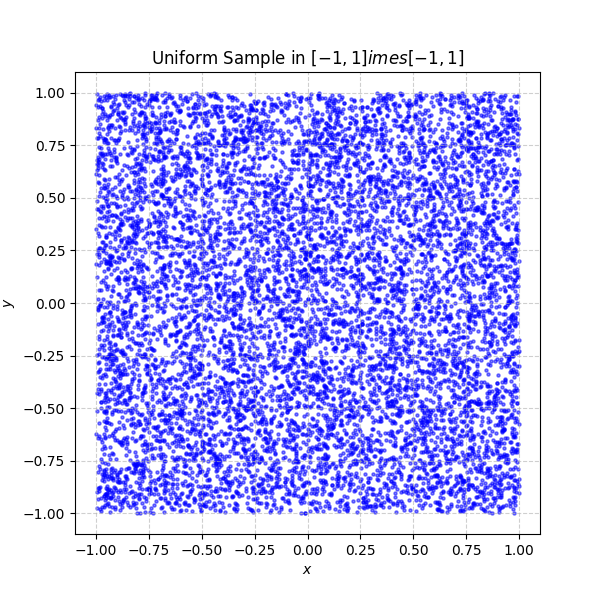
\includegraphics[width=\textwidth]{tex/ims/unixy.png}
    \end{minipage}
    \begin{minipage}{.4\textwidth}
    \centering
    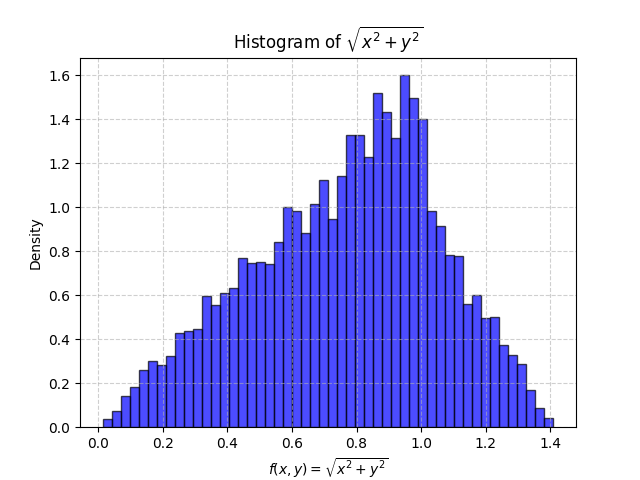
\includegraphics[width=\textwidth]{tex/ims/unirad.png}
    
    \end{minipage}
     \caption{A function on a uniform distribution need not yield a uniform distribution. An easy example is the radius function.}
             \end{figure}

So, the first row makes sense. 
For the single channel phase space in the bottom row, the distribution on the left is very narrowly distributed to 90GeV. This is because we reject a lot of points in order to only include momenta relevant to the process. In theory, multiplying but the Jacobian, which encodes this change of phase region, should yield in the bottom right a distribution that looks like the top row. Clearly, this doesn't seem to be the case. This is because we don't have enough statistics to accurately reproduce the top row - we have rejected a large number of samples. If we increase the width of the $Z$ boson from 60Gev to say, 6000GeV, we can see the distributions start to match a bit more closely, as we are rejecting fewer points.

\begin{figure}[H]
    \centering
    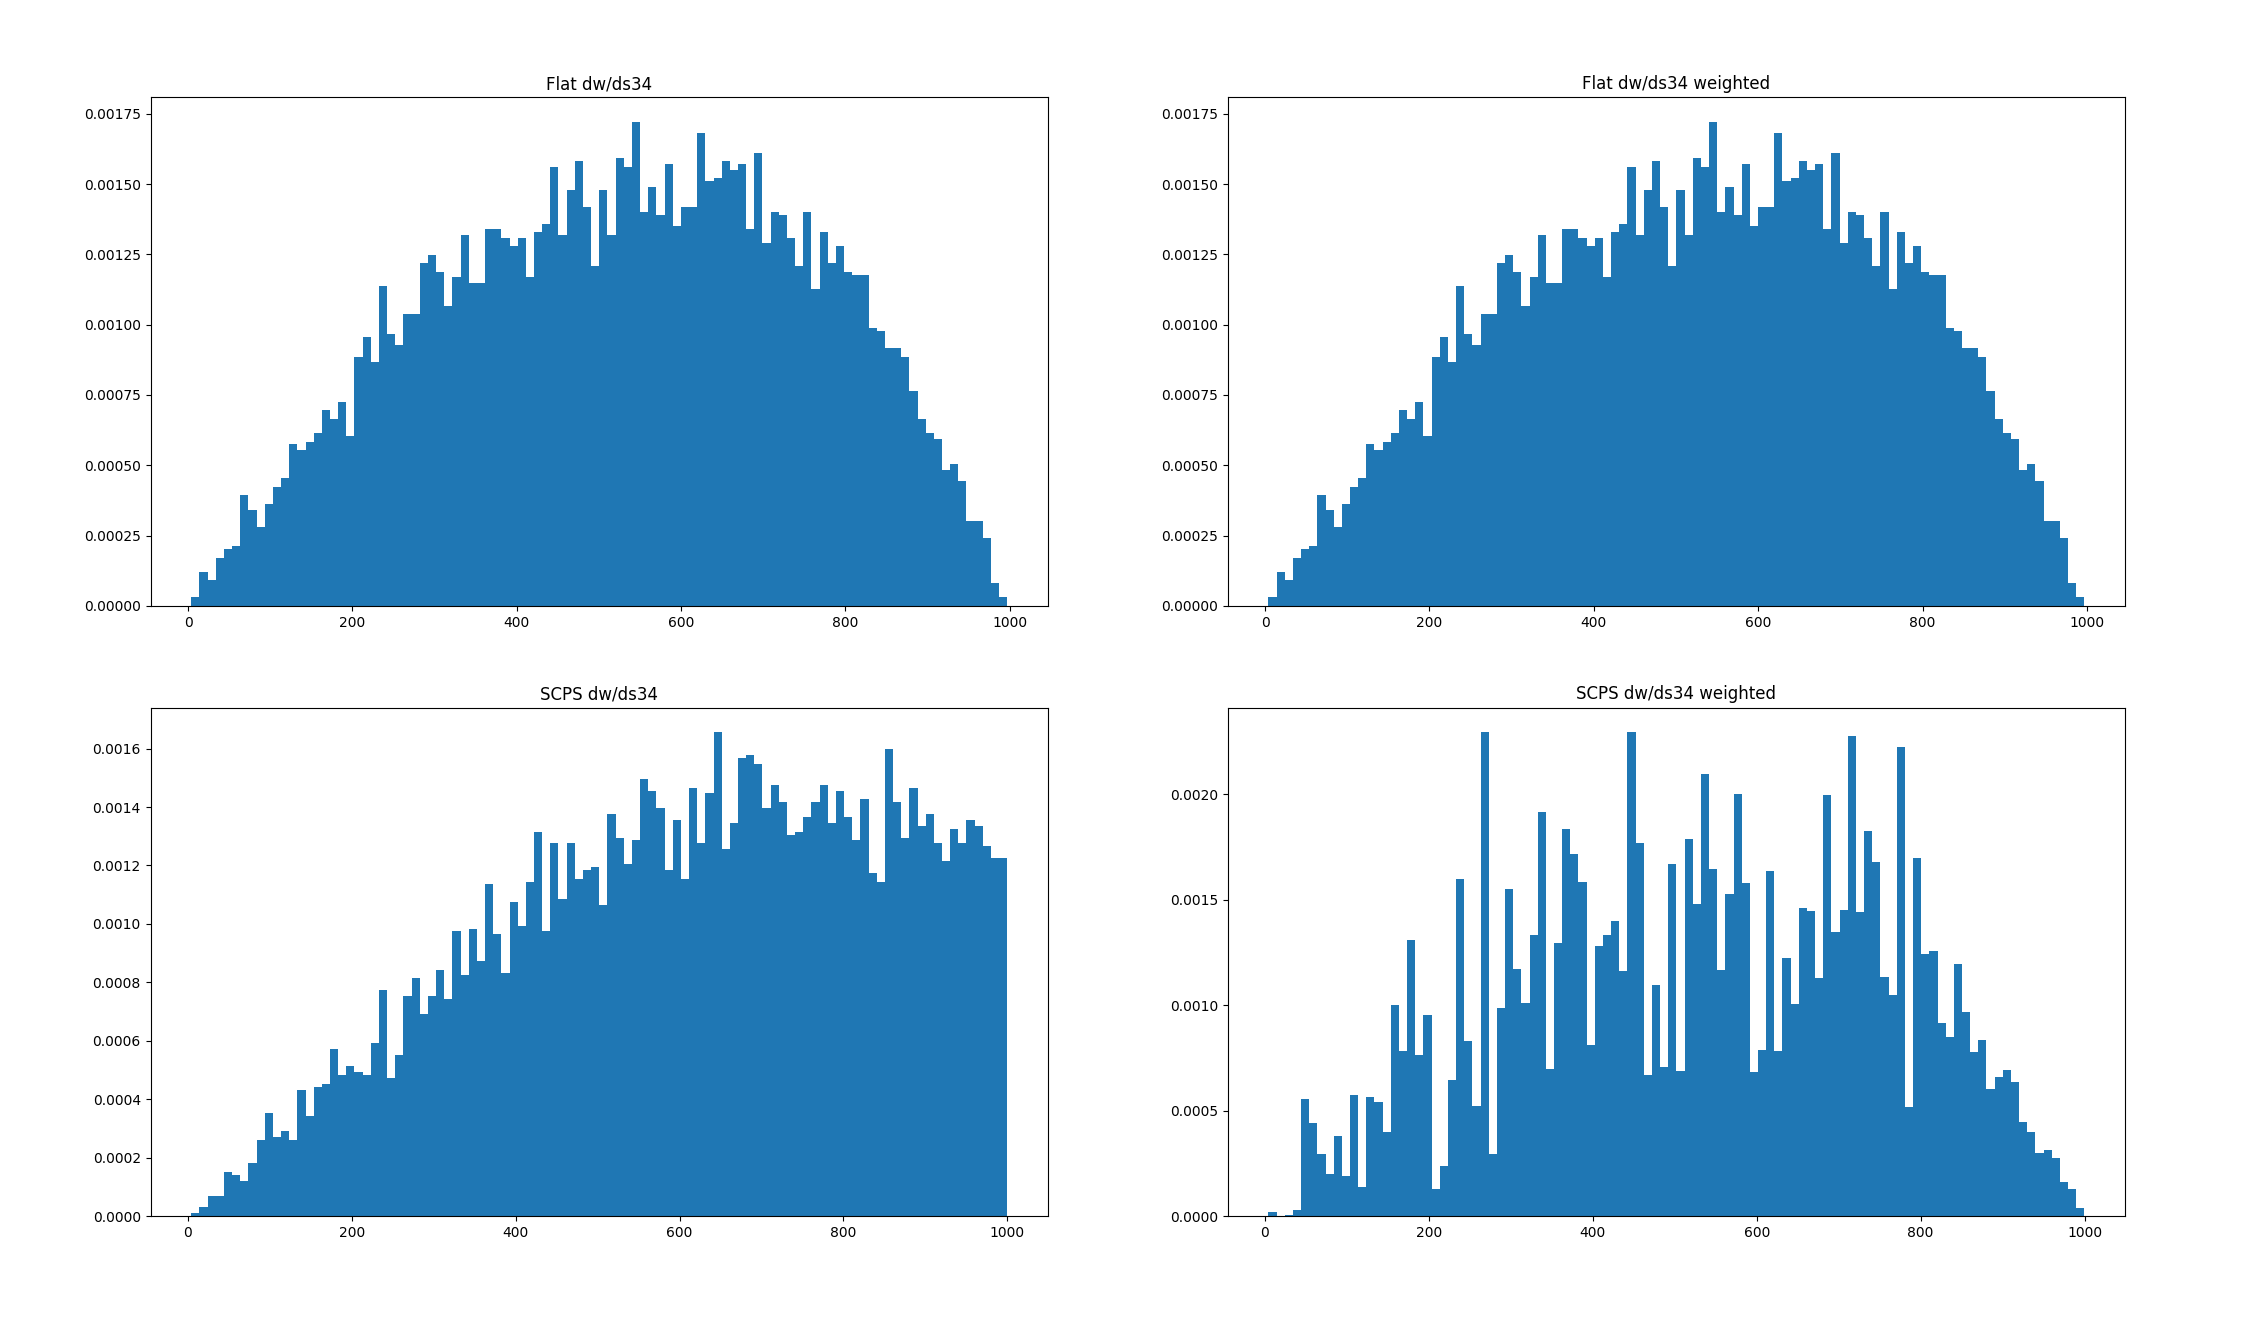
\includegraphics[width=0.75\linewidth]{tex/ims/phasespace2.png}
    \caption{Phase Space Sampling with the $Z$ boson with mass 150GeV and width 6000GeV. The reweighted distribution on the bottom right starts to look more like the top row, as with this width we reject fewer points and thus have better statistics.}
    \label{fig:phase2}
\end{figure}



% We can do this using Symbolica.



% \bibliographystyle{unsrt}
% \bibliography{refs}
\end{document}
